\documentclass{article}
\usepackage{amsmath}
\usepackage{tikz}
\usetikzlibrary{matrix}
\usepackage{ifthen}

\newcommand{\wh}{\textcolor{red}{\boldsymbol{w}_h}}
\newcommand{\wl}{\textcolor{black}{\boldsymbol{w}_l}}

\begin{document}

\begin{figure}[htbp]
    \centering
    \begin{subfigure}[b]{0.3\textwidth}
        \centering
        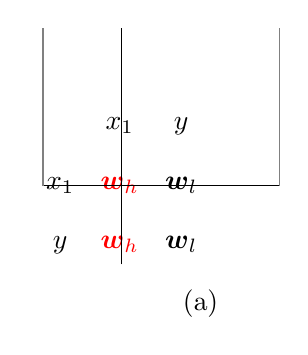
\begin{tikzpicture}
            \matrix[matrix of math nodes, row sep=3mm, column sep=1mm] {
                & x_1 & y\\
                x_1 & \wh & \wl\\
                y & \wh & \wl\\
            };
            \draw [-] (0,-1) -- (0,2);
            \draw [-] (-1,0) -- (2,0);
            \draw [gray] (-1,0) -- (-1,2);
            \draw [gray] (2,0) -- (2,2);
            \node at (1,-1.5) {(a)};
        \end{tikzpicture}
        \caption{}
    \end{subfigure}
    ~
    \begin{subfigure}[b]{0.3\textwidth}
        \centering
        \begin{tikzpicture}
            \matrix[matrix of math nodes, row sep=3mm, column sep=1mm] {
                & x_1 & x_2 & y\\
                x_1 & \wl & \wh & \wl\\
                x_2 & \wh & \wl & \wl\\
                y & \wh & \wl & \wl\\
            };
            \draw [-] (0,-1) -- (0,4);
            \draw [-] (-1,0) -- (4,0);
            \draw [gray] (-1,0) -- (-1,4);
            \draw [gray] (4,0) -- (4,4);
            \node at (1,-1.5) {(b)};
        \end{tikzpicture}
    \caption{}
    \end{subfigure}
    ~
    \begin{subfigure}[b]{0.3\textwidth}
        \centering
        \begin{tikzpicture}
            \matrix[matrix of math nodes, row sep=3mm, column sep=1mm] {
                & x_1 & x_2 & x_3 & y\\
                x_1, x_1 & \wl & \wh & \wl & \wl\\
                x_1, x_2 & \wl & \wl & \wh & \wl\\
                x_1, x_3 & \wh & \wl & \wl & \wl\\
                x_1, y & \wh & \wl & \wl & \wl\\
                & \vdots & & & \\
            };
            \draw [-] (0,-1) -- (0,6);
            \draw [-] (-1,0) -- (5,0);
            \draw [gray] (-1,0) -- (-1,6);
            \draw [gray] (5,0) -- (5,6);
            \node at (1,-1.5) {(c)};
        \end{tikzpicture}
    \caption{}
    \end{subfigure}
    \caption{Transition probability matrices for node (a), edge (b), and path ($l=2$) (c) hypotheses, where $\boldsymbol{w}_h \geq \boldsymbol{w}_l > 0$ denote transition probabilities. $x_i$ represents nodes in $\mathcal{G}$ satisfying the $i$-th node modifier on $\mathcal{P}$, while $y$ represents nodes not satisfying any node modifier on $\mathcal{P}$. (a) and (b) involve 1st-order random walks, whereas (c) involves 2nd-order random walks because the probability of selecting the next node depends on both the current and previous nodes.}
\end{figure}

\end{document}